\documentclass[12pt,a4paper]{report}

\usepackage[utf8]{inputenc}
\usepackage[T1]{fontenc}
\usepackage{lmodern}
\usepackage[a4paper,margin=1in]{geometry}
\usepackage{graphicx}
\usepackage{booktabs}
\usepackage{tabularx}
\usepackage{longtable}
\usepackage{array}
\usepackage{enumitem}
\usepackage{xcolor}
\usepackage{hyperref}
\usepackage{float}
\usepackage{caption}
\usepackage{listings}
\usepackage{setspace}
\usepackage{fancyhdr}
\usepackage{titlesec}

\graphicspath{{../images/}}
\setstretch{1.15}
\setlength{\parskip}{0.45em}
\setlength{\parindent}{0pt}

\hypersetup{
  colorlinks=true,
  linkcolor=blue!60!black,
  urlcolor=blue!60!black,
  citecolor=blue!60!black,
  pdftitle={Midterm Report - RAG Web UI},
  pdfauthor={Student Name},
  pdfsubject={Midterm implementation report},
  pdfkeywords={RAG, FastAPI, Next.js, ChromaDB, MinIO, admin dashboard, expert review}
}

\pagestyle{fancy}
\fancyhf{}
\fancyhead[L]{RAG Web UI Midterm Report}
\fancyhead[R]{\thepage}
\renewcommand{\headrulewidth}{0.4pt}

\titleformat{\chapter}{\normalfont\huge\bfseries}{\thechapter.}{0.75em}{}
\titleformat{\section}{\normalfont\Large\bfseries}{\thesection}{0.75em}{}
\titleformat{\subsection}{\normalfont\large\bfseries}{\thesubsection}{0.75em}{}

\lstdefinestyle{projectstyle}{
  basicstyle=\ttfamily\small,
  breaklines=true,
  frame=single,
  columns=fullflexible,
  keepspaces=true,
  backgroundcolor=\color{black!2},
  rulecolor=\color{black!15}
}

\begin{document}

\begin{titlepage}
\centering
\vspace*{1.2cm}

{\Huge\bfseries Midterm Report\par}
\vspace{0.3cm}
{\LARGE RAG Web UI for Internal Knowledge Retrieval and Question Answering\par}
\vspace{1cm}


\includegraphics[width=0.9\textwidth]{github-cover-new.png}\par
\vspace{1cm}

\begin{tabular}{p{0.28\textwidth}p{0.6\textwidth}}
\textbf{Course:} & Midterm Project Report \\
\textbf{Project Title:} & RAG Web UI \\
\textbf{Student Name:} & \textit{Fill in your name} \\
\textbf{Student ID:} & \textit{Fill in your student ID} \\
\textbf{Supervisor / Lecturer:} & \textit{Fill in lecturer name} \\
\textbf{Submission Date:} & \textit{Fill in date} \\
\end{tabular}

\vfill

{\large Department / Faculty / University\par}
\end{titlepage}

\tableofcontents
\listoffigures
\listoftables
\clearpage

\chapter{Executive Summary}

This report presents the midterm implementation status of \textbf{RAG Web UI}, a web-based Retrieval-Augmented Generation system designed for internal document question answering. The project combines a modern web frontend, a FastAPI backend, a vector database, object storage, and large language model integration to provide reliable answers grounded in enterprise documents.

The original project already supported document upload, knowledge base management, and retrieval-based chat. During this midterm phase, the system was extended substantially to better fit a real organizational workflow. The major additions include user profiles, document-level permissions, a feedback system, an admin dashboard, analytics, expert answer override, improved chat interaction, audit logging, and a safer first-run admin bootstrap mechanism.

The implementation goal of this phase was not only to add features, but also to improve system operability, trustworthiness, and governance. In practical terms, the system now supports three clearer operational roles:
\begin{itemize}[leftmargin=1.5em]
\item \textbf{User}: asks questions, reviews chat history, accesses authorized documents, and evaluates answer quality.
\item \textbf{Expert}: manually reviews and corrects answers that users flagged as inaccurate.
\item \textbf{Admin / Super Admin}: manages users, documents, permissions, system settings, alerts, and quality workflows.
\end{itemize}

The project is currently functional as a multi-service Docker deployment and includes both user-facing and administrative workflows. The system is appropriate for a midterm milestone because the core product loop is already in place: ingest documents, retrieve relevant content, generate cited answers, collect feedback, escalate low-quality responses to experts, and monitor the entire system through an administrative interface.

\chapter{Project Background and Objectives}

\section{Problem Statement}

Organizations often store important internal knowledge in scattered documents such as PDFs, Word files, text files, and internal reports. Employees need fast access to accurate information, but manually searching large collections is inefficient and error-prone. A question answering system backed by internal documents can reduce this friction; however, such a system must also address accountability, document permissions, answer quality, and administrative oversight.

The project therefore targets the following practical problem:

\textit{How can we build a web-based question answering system that retrieves information from internal documents, generates grounded responses, and still provides sufficient controls for security, monitoring, and human correction?}

\section{Project Objectives}

The main objectives of the project are:
\begin{itemize}[leftmargin=1.5em]
\item Build a Retrieval-Augmented Generation platform for internal document search and question answering.
\item Support document ingestion, storage, indexing, and retrieval from multiple knowledge bases.
\item Provide a clean chat interface with answer citations.
\item Enforce access control so users only see authorized knowledge.
\item Collect feedback from users to evaluate answer quality.
\item Allow expert intervention when a chatbot answer is flagged as incorrect.
\item Provide admins with tools for user management, content governance, monitoring, and system configuration.
\end{itemize}

\section{Scope of the Midterm Phase}

The midterm phase focused on delivering a usable end-to-end product increment, including:
\begin{itemize}[leftmargin=1.5em]
\item stable backend and frontend deployment,
\item user authentication and profile management,
\item knowledge base and document management,
\item answer generation using retrieved context,
\item feedback collection and expert override,
\item admin analytics and operational controls,
\item technical fixes required to keep the stack deployable.
\end{itemize}

\chapter{System Overview}

\section{High-Level Architecture}

The project follows a frontend-backend separated architecture with supporting infrastructure services. The main components are:
\begin{itemize}[leftmargin=1.5em]
\item \textbf{Frontend}: Next.js 14 + TypeScript + Tailwind CSS dashboard application.
\item \textbf{Backend}: FastAPI REST API with JWT-based authentication.
\item \textbf{Relational Database}: MySQL for users, chats, metadata, permissions, feedback, and admin logs.
\item \textbf{Vector Store}: ChromaDB by default, with a factory-based path for alternative vector databases such as Qdrant.
\item \textbf{Object Storage}: MinIO for uploaded source documents.
\item \textbf{Reverse Proxy}: Nginx for service exposure.
\item \textbf{LLM Layer}: OpenAI, DeepSeek, or Ollama through configurable factories.
\end{itemize}

\section{Deployment Topology}

The Docker deployment in the project composes the following services:
\begin{table}[H]
\centering
\begin{tabularx}{\textwidth}{>{\bfseries}l l X}
\toprule
Service & Technology & Responsibility \\
\midrule
frontend & Next.js & User interface, dashboards, chat, admin pages \\
backend & FastAPI & APIs, business logic, authentication, orchestration \\
db & MySQL 8 & Transactional data and metadata \\
chromadb & ChromaDB & Embedding storage and similarity retrieval \\
minio & MinIO & File storage for uploaded documents \\
nginx & Nginx & Reverse proxy and routing \\
\bottomrule
\end{tabularx}
\caption{Main services in the deployed system}
\end{table}

\section{RAG Processing Flow}

The implemented question answering workflow is:
\begin{enumerate}[leftmargin=1.5em]
\item A user selects one or more knowledge bases and asks a question.
\item The backend retrieves prior chat history for conversational context.
\item The system builds embeddings and queries the vector store for relevant chunks.
\item Retrieved chunks are passed into the LLM prompt together with system instructions.
\item The answer is generated with citations derived from retrieved context.
\item The final answer is streamed to the frontend and stored in chat history.
\item The user can rate the answer, and negative feedback can trigger expert review.
\end{enumerate}

\section{Illustrative Screenshots}

\begin{figure}[H]
\centering
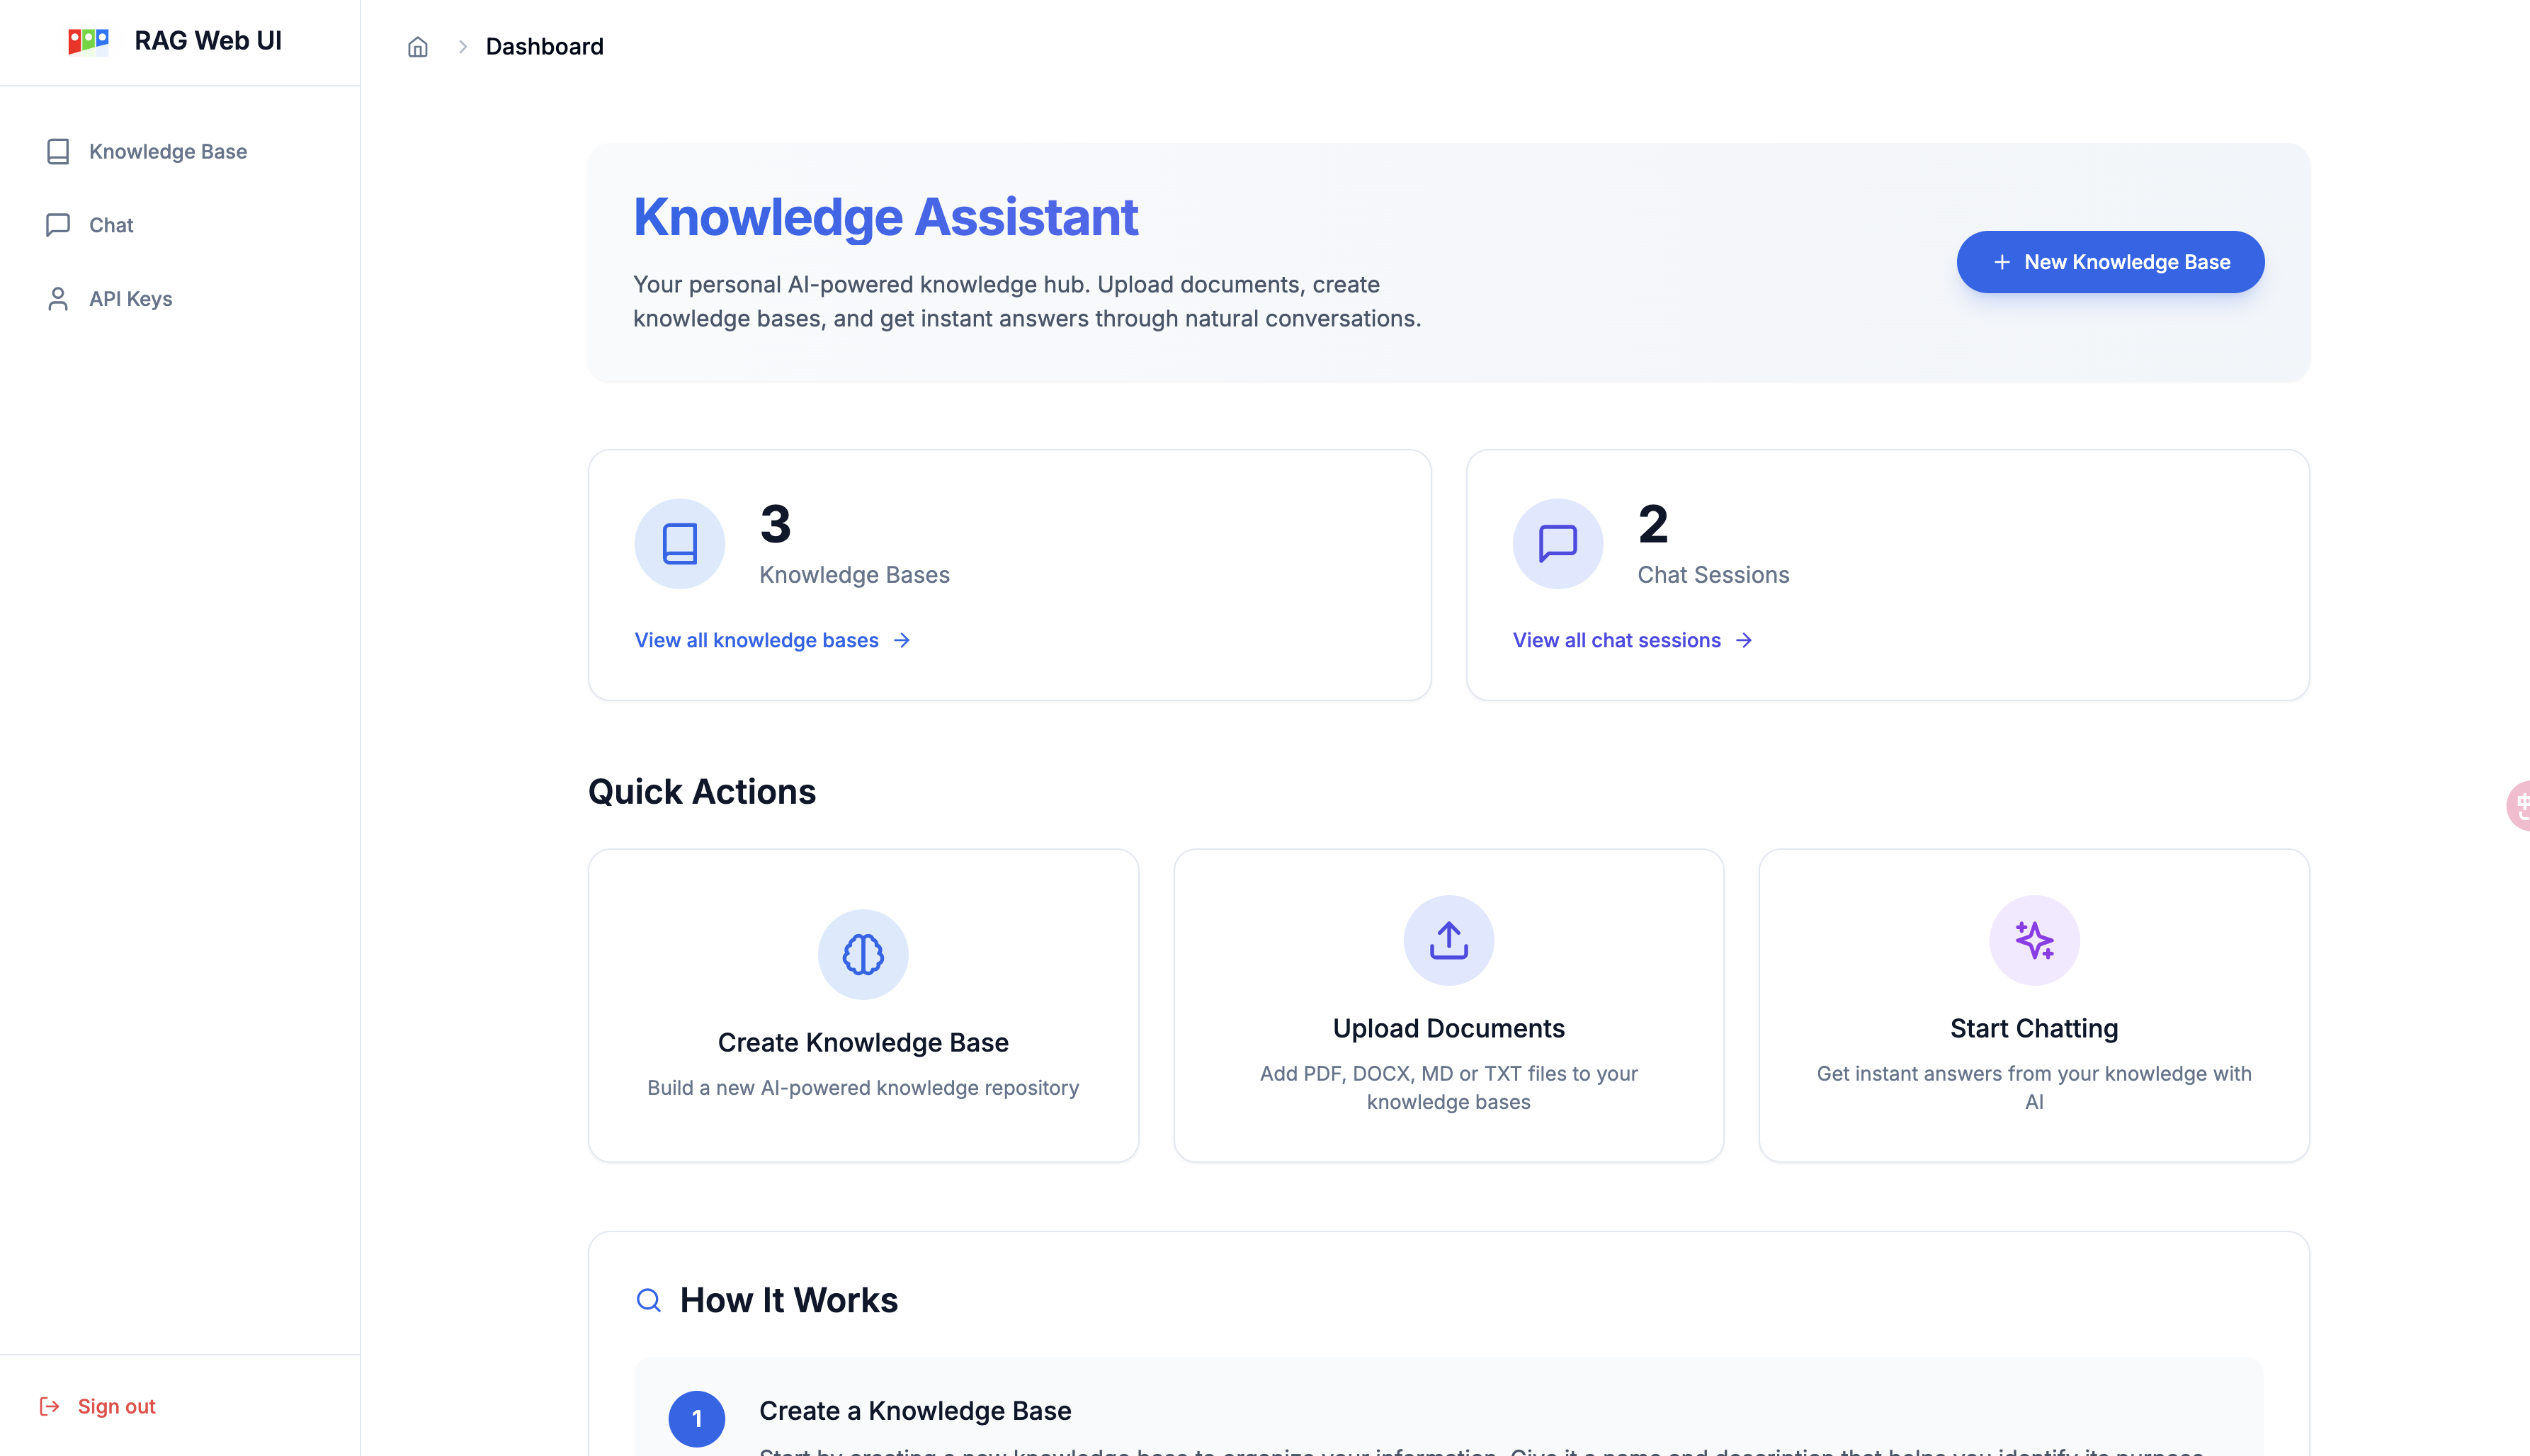
\includegraphics[width=0.9\textwidth]{screenshot1.png}
\caption{Knowledge base management interface}
\end{figure}

\begin{figure}[H]
\centering
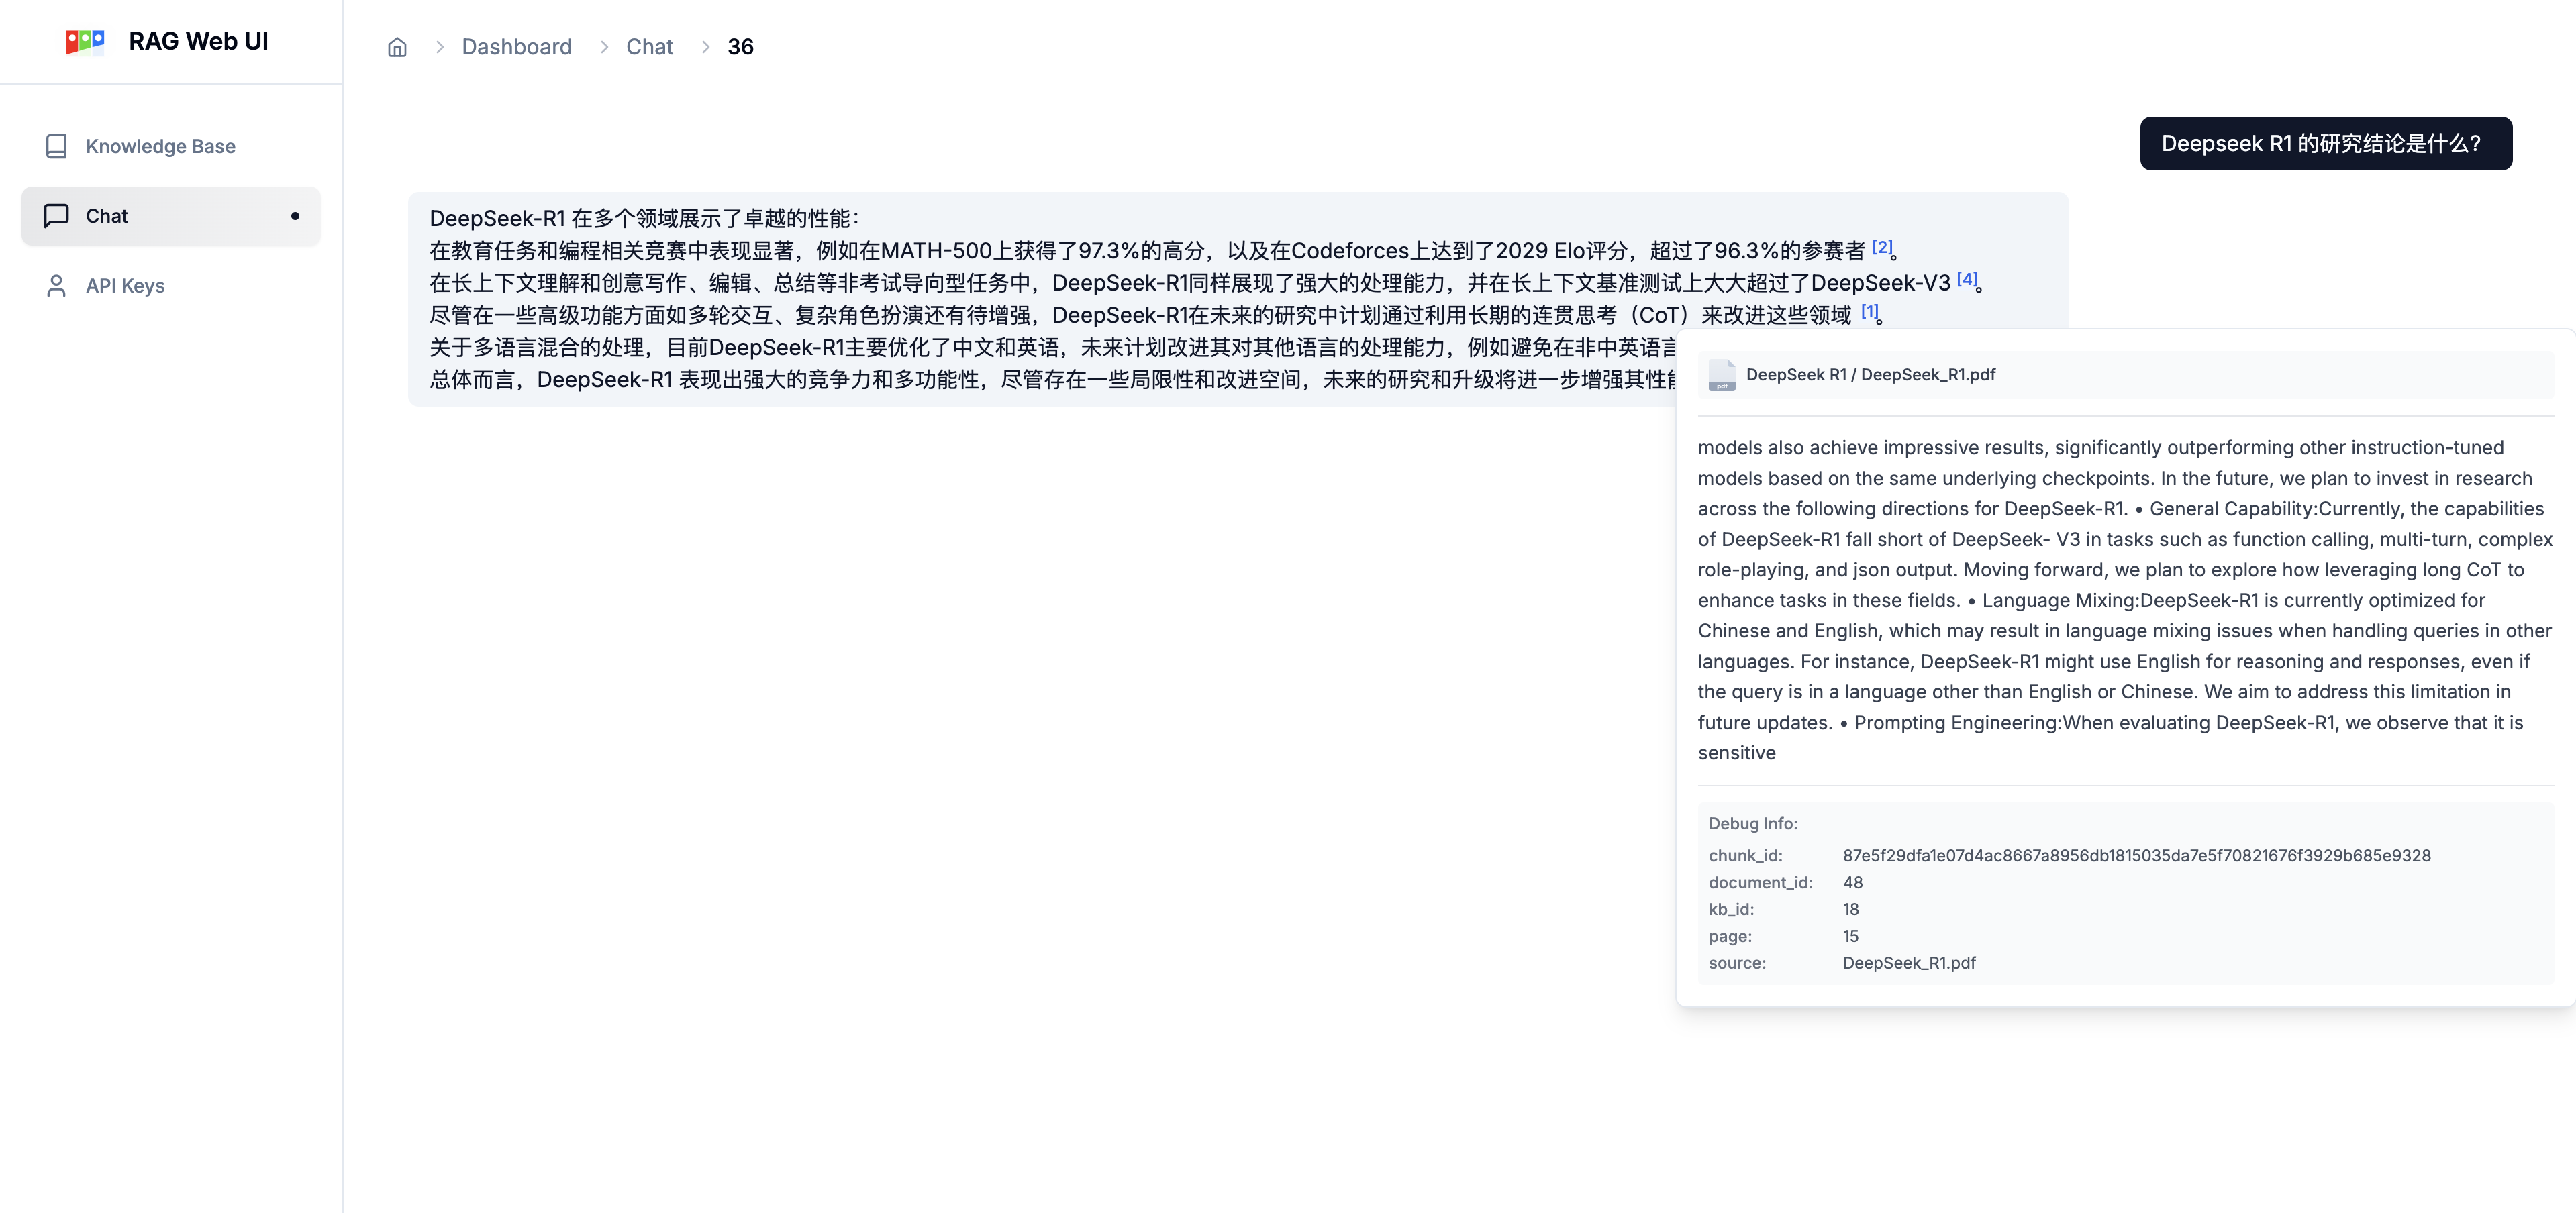
\includegraphics[width=0.9\textwidth]{screenshot4.png}
\caption{Chat interface with answer generation and citations}
\end{figure}

\begin{figure}[H]
\centering
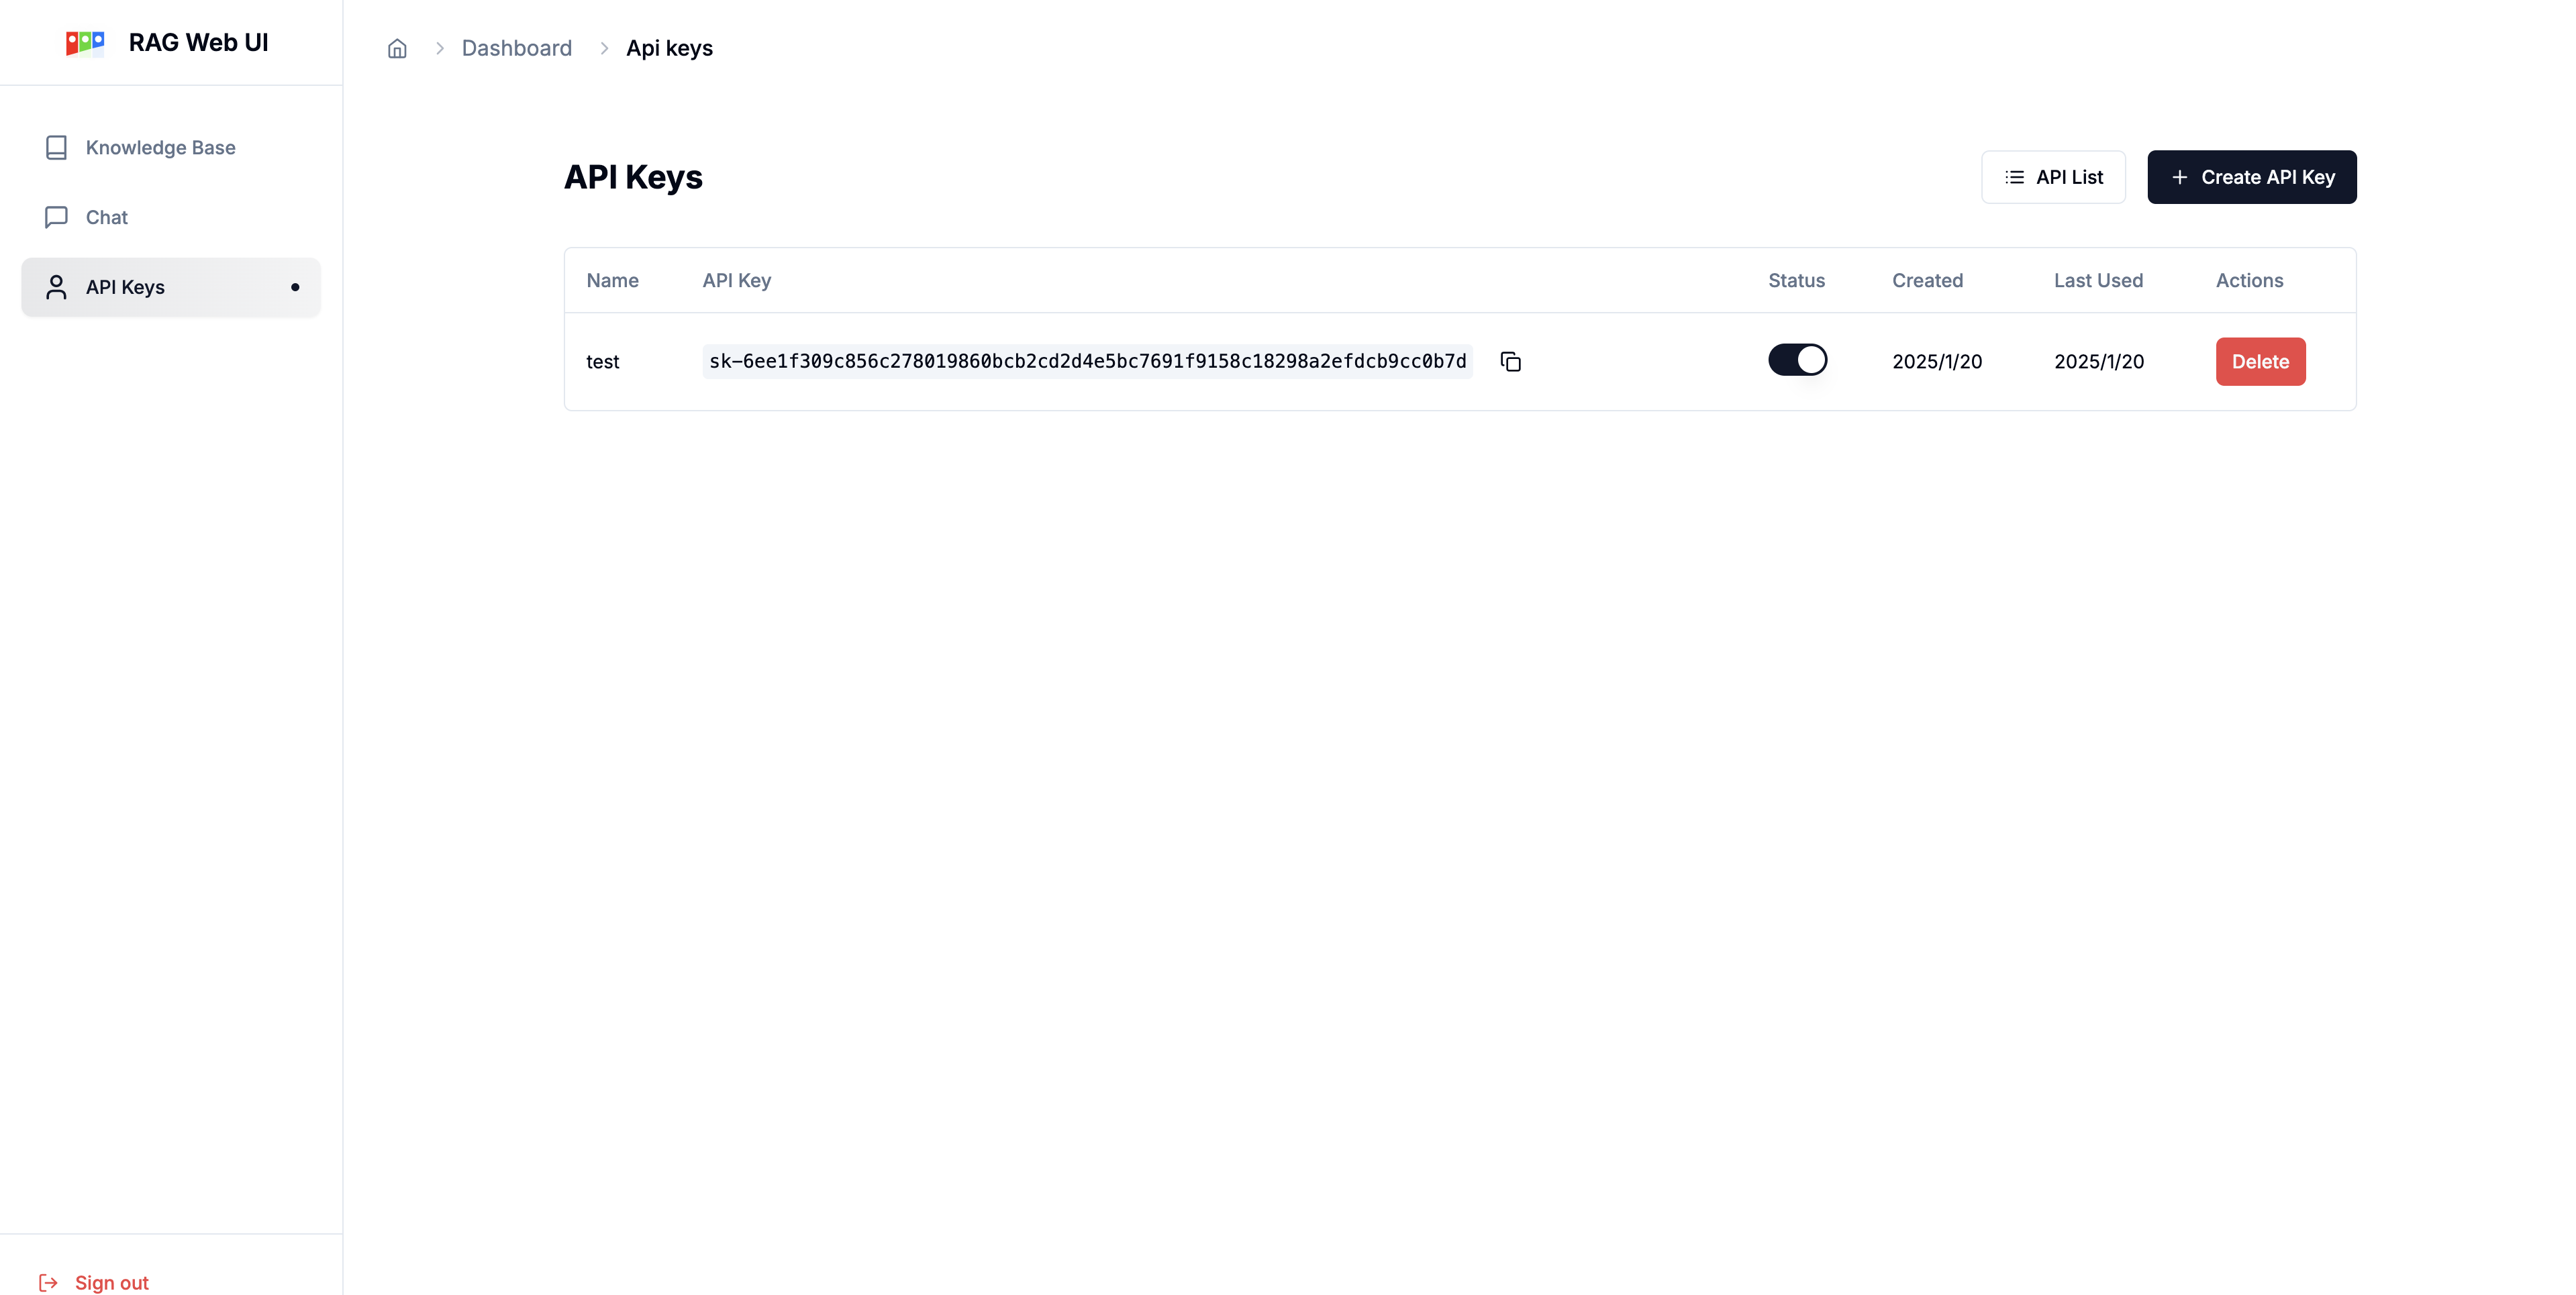
\includegraphics[width=0.9\textwidth]{screenshot5.png}
\caption{Analytics and monitoring dashboard area}
\end{figure}

\chapter{Technology Stack}

\section{Backend Stack}

\begin{itemize}[leftmargin=1.5em]
\item \textbf{Python / FastAPI}: API framework for authentication, chat, knowledge base, feedback, analytics, and admin routes.
\item \textbf{SQLAlchemy}: ORM for relational models and database access.
\item \textbf{Alembic}: database schema migration management.
\item \textbf{LangChain}: orchestration for retriever and answer generation chains.
\item \textbf{MySQL Connector}: backend database driver.
\item \textbf{JWT + OAuth2 password flow}: token-based authentication.
\end{itemize}

\section{Frontend Stack}

\begin{itemize}[leftmargin=1.5em]
\item \textbf{Next.js 14}: application framework with App Router.
\item \textbf{TypeScript}: static typing for UI and API payloads.
\item \textbf{Tailwind CSS}: styling and responsive dashboard layout.
\item \textbf{Lucide Icons and custom UI components}: navigation and UI composition.
\end{itemize}

\section{Infrastructure and Storage}

\begin{itemize}[leftmargin=1.5em]
\item \textbf{MinIO}: object storage for uploaded source files.
\item \textbf{ChromaDB}: vector store used for retrieval.
\item \textbf{Docker Compose}: multi-service development and deployment environment.
\item \textbf{Nginx}: reverse proxy in front of frontend and backend.
\end{itemize}

\chapter{Data Model and Role Design}

\section{Core Data Entities}

The system data model is centered around the following entities:
\begin{itemize}[leftmargin=1.5em]
\item \textbf{User}: authentication identity, role, profile data, flags, and account status.
\item \textbf{KnowledgeBase}: logical collection of internal documents.
\item \textbf{Document}: uploaded file metadata, status, access settings, indexing metadata.
\item \textbf{Chat}: a conversation session owned by a user.
\item \textbf{Message}: user or assistant messages within a chat.
\item \textbf{MessageFeedback}: user feedback attached to assistant answers.
\item \textbf{MessageOverride}: expert-authored replacement for an assistant answer.
\item \textbf{ManualQAEntry}: manually curated question-answer pairs.
\item \textbf{AuditLog / AccessLog / SystemAlert / SystemConfig}: governance and monitoring entities.
\end{itemize}

\section{Role Separation}

The project now separates roles more clearly than the original baseline:
\begin{table}[H]
\centering
\begin{tabularx}{\textwidth}{>{\bfseries}l X}
\toprule
Role & Main Responsibilities \\
\midrule
User & Ask questions, view chat history, review accessible documents, provide answer feedback \\
Expert & Review flagged answers assigned for manual correction and submit expert overrides \\
Admin & Manage users, permissions, documents, analytics, alerts, manual Q\&A, and quality workflow \\
Super Admin & Full admin capabilities including sensitive or destructive operations \\
\bottomrule
\end{tabularx}
\caption{Operational role model used by the system}
\end{table}

\chapter{Midterm Implementation Work}

\section{Baseline Capabilities Inherited from the Project}

Before the extension work, the repository already supported:
\begin{itemize}[leftmargin=1.5em]
\item user registration and login,
\item document upload and knowledge base creation,
\item vector indexing and retrieval,
\item question answering over uploaded content,
\item API key management,
\item basic dashboard pages.
\end{itemize}

\section{Major Features Implemented During This Phase}

\subsection{User Account Profiles}

The user model was extended to support richer profile information and clearer account state handling. The implementation includes:
\begin{itemize}[leftmargin=1.5em]
\item \texttt{full\_name}, \texttt{bio}, and \texttt{avatar\_url} fields,
\item role metadata,
\item account suspension fields,
\item per-user feature flags,
\item profile retrieval and update endpoints.
\end{itemize}

This work improves usability and also supports more advanced role-aware navigation on the frontend.

\subsection{Document Permissions and Knowledge Governance}

To better support internal document protection, permission entities were added for:
\begin{itemize}[leftmargin=1.5em]
\item knowledge-base-level access,
\item document-level access,
\item document metadata such as category, department, sensitivity, and access level.
\end{itemize}

These additions make the system more suitable for departmental or restricted-content deployment scenarios.

\subsection{Feedback System}

A dedicated answer feedback mechanism was added so users can evaluate assistant responses. The system supports:
\begin{itemize}[leftmargin=1.5em]
\item positive or negative feedback on assistant messages,
\item optional comments,
\item status transitions such as submitted, flagged, assigned, and resolved,
\item backend persistence for reporting and follow-up.
\end{itemize}

This is a key quality assurance feature because it transforms passive usage into measurable signal.

\subsection{Admin Dashboard}

The admin workspace was implemented as a central operational console. It provides views and actions for:
\begin{itemize}[leftmargin=1.5em]
\item user creation and role management,
\item activation, deactivation, suspension, and unsuspension,
\item document and knowledge base visibility,
\item reindex actions,
\item system alerts and audit logs,
\item manual Q\&A management,
\item flagged answer assignment to experts,
\item system configuration.
\end{itemize}

\subsection{Analytics}

The project now includes administrative analytics such as:
\begin{itemize}[leftmargin=1.5em]
\item total users, chats, questions, documents, and feedback count,
\item seven-day activity trend,
\item top users by chat volume,
\item frequent topics based on recent questions,
\item peak usage hours,
\item answer feedback summary,
\item document query effectiveness.
\end{itemize}

These metrics help the project move from a demo system toward an operable product.

\subsection{Expert Answer Override}

One of the most important additions in this phase is the expert escalation workflow. The implemented logic is:
\begin{enumerate}[leftmargin=1.5em]
\item A user marks an answer as inaccurate.
\item The feedback status becomes \texttt{flagged}.
\item An admin views flagged answers and assigns the case to an expert.
\item The expert sees the case in a dedicated review queue.
\item The expert submits a corrected manual answer.
\item The manual answer is stored as an override and the feedback status becomes \texttt{resolved}.
\end{enumerate}

This workflow addresses a real limitation of automated systems: not every answer should remain purely machine-generated when correctness matters.

\subsection{Improved Chat Conversation Experience}

The chat interface was improved significantly to feel smoother and more natural. Previously, a user had to refresh or navigate away and back before the new answer became visible. The updated implementation now:
\begin{itemize}[leftmargin=1.5em]
\item appends the user message immediately,
\item creates an optimistic assistant placeholder,
\item streams assistant output incrementally from the backend,
\item updates citations as the answer accumulates,
\item refreshes message state after streaming completes.
\end{itemize}

This change improves the perceived responsiveness and usability of the system.

\subsection{Safer Admin Bootstrap}

To simplify first-time setup, a safer environment-based admin bootstrap flow was added. The backend can now create or update the initial administrator from \texttt{.env} values during startup. This was added to reduce manual setup friction and to avoid repeated terminal command issues.

\chapter{Implementation Details}

\section{Backend Modules Added or Extended}

The following areas were extended during this phase:
\begin{table}[H]
\centering
\begin{tabularx}{\textwidth}{>{\ttfamily}l X}
\toprule
Module / Area & Purpose \\
\midrule
backend/app/api/api\_v1/auth.py & authentication, profile access, admin and expert guards \\
backend/app/api/api\_v1/feedback.py & user answer feedback and expert override workflow \\
backend/app/api/api\_v1/admin.py & administrative APIs, analytics, alerts, user management \\
backend/app/api/api\_v1/analytics.py & analytics endpoints for dashboard usage \\
backend/app/models/user.py & richer user profile and role fields \\
backend/app/models/chat.py & feedback, override, and expert assignment data structures \\
backend/app/models/knowledge.py & permission and metadata support for governed documents \\
backend/app/models/admin.py & audit logs, access logs, alerts, system config, manual Q\&A \\
backend/app/services/chat\_service.py & streaming answer generation and manual answer shortcut \\
backend/app/startup/admin\_bootstrap.py & startup-based admin account provisioning \\
\bottomrule
\end{tabularx}
\caption{Key backend areas modified in the midterm phase}
\end{table}

\section{Frontend Modules Added or Extended}

The frontend was updated to reflect the new operational model:
\begin{table}[H]
\centering
\begin{tabularx}{\textwidth}{>{\ttfamily}l X}
\toprule
Page / Component & Purpose \\
\midrule
frontend/src/app/dashboard/admin/page.tsx & admin workspace UI \\
frontend/src/app/dashboard/analytics/page.tsx & analytics dashboard \\
frontend/src/app/dashboard/profile/page.tsx & user profile editing \\
frontend/src/app/dashboard/expert-review/page.tsx & expert queue and manual correction UI \\
frontend/src/app/dashboard/chat/[id]/page.tsx & smooth streaming chat and feedback UI \\
frontend/src/components/layout/dashboard-layout.tsx & role-based navigation for user, expert, and admin \\
frontend/src/components/knowledge-base/document-list.tsx & document permissions and visibility management \\
\bottomrule
\end{tabularx}
\caption{Key frontend areas modified in the midterm phase}
\end{table}

\section{Database Evolution}

The data model was expanded through new schema migrations to support:
\begin{itemize}[leftmargin=1.5em]
\item user profile fields,
\item knowledge base and document permissions,
\item feedback and override metadata,
\item audit and access logging,
\item admin system settings and alerts,
\item expert assignment workflow.
\end{itemize}

\chapter{Workflow Design}

\section{User Workflow}

The user-facing workflow is now:
\begin{enumerate}[leftmargin=1.5em]
\item Log in to the web application.
\item Access permitted knowledge bases and documents.
\item Start or continue a conversation with the chatbot.
\item Receive answers grounded in retrieved document content.
\item Review chat history and citations.
\item Provide thumbs-up or thumbs-down feedback on each answer.
\end{enumerate}

\section{Admin Workflow}

The admin workflow includes:
\begin{enumerate}[leftmargin=1.5em]
\item Create and manage user accounts.
\item Assign roles such as user, expert, admin, and super admin.
\item Monitor document usage, alerts, and failed access attempts.
\item Manage knowledge bases, documents, and reindexing.
\item View flagged answers and assign them to experts.
\item Configure answer settings and feedback routing behavior.
\end{enumerate}

\section{Expert Workflow}

The expert workflow is:
\begin{enumerate}[leftmargin=1.5em]
\item Open the expert review queue.
\item Review the user question, original chatbot answer, and user complaint.
\item Submit a corrected expert answer.
\item Resolve the flagged answer case.
\end{enumerate}

\chapter{Challenges Encountered and Solutions Applied}

\section{Build and Configuration Issues}

Several deployment and build issues were identified and fixed during this phase:
\begin{itemize}[leftmargin=1.5em]
\item Deprecated Next.js configuration keys were updated to the current format.
\item A frontend page contained invalid UTF-8 bytes and had to be normalized.
\item TypeScript type mismatches in feedback status handling were corrected.
\item Tailwind plugin warnings were cleaned up by removing redundant configuration.
\end{itemize}

\section{Backend Stability Issues}

The backend also required multiple runtime fixes:
\begin{itemize}[leftmargin=1.5em]
\item A startup migration checker compared the wrong revisions and was corrected.
\item A missing database migration caused ``unknown column'' SQL errors after model expansion.
\item A Python f-string escape issue in the streaming service caused container startup failure and was replaced with safe JSON encoding.
\item SQLAlchemy relationship ambiguity between feedback owner and expert assignee was resolved with explicit foreign key definitions.
\end{itemize}

\section{Operational Usability Issues}

The project also faced practical developer-experience issues:
\begin{itemize}[leftmargin=1.5em]
\item PowerShell command syntax made multi-line bootstrap commands inconvenient.
\item The initial admin setup path was too error-prone for first-time use.
\item Some user interface labels and text consistency needed cleanup and standardization.
\end{itemize}

These issues were addressed by improving startup bootstrap behavior, normalizing the UI to English, and strengthening the deployment workflow.

\chapter{Testing and Verification}

\section{Verification Methods Used}

During implementation, the following validation steps were applied:
\begin{itemize}[leftmargin=1.5em]
\item Python module compilation checks using \texttt{py\_compile} and \texttt{compileall}.
\item Frontend build validation through \texttt{pnpm build}.
\item Docker-based service startup testing.
\item Log inspection for backend runtime errors and authentication flow issues.
\item Manual verification of role-based dashboard routing and chat flow behavior.
\end{itemize}

\section{Validated Outcomes}

The midterm work achieved the following verified outcomes:
\begin{itemize}[leftmargin=1.5em]
\item backend model and service modules compile successfully,
\item frontend configuration and encoding issues were resolved,
\item chat streaming updates appear without requiring page refresh,
\item expert assignment and manual answer paths are wired end-to-end,
\item admin bootstrap can now be driven from environment variables.
\end{itemize}

\section{Remaining Validation Work}

Although the system is functional, several areas still deserve stronger validation in the next phase:
\begin{itemize}[leftmargin=1.5em]
\item end-to-end automated tests,
\item permission boundary testing for retrieval-layer enforcement,
\item performance testing with larger document collections,
\item user acceptance testing with realistic internal content,
\item notification integrations such as email, Slack, or Microsoft Teams.
\end{itemize}

\chapter{Current Progress Assessment}

\section{What Has Been Completed}

At the midterm milestone, the project already includes:
\begin{itemize}[leftmargin=1.5em]
\item a working multi-service deployment,
\item document upload and indexing,
\item retrieval-based conversational question answering,
\item citation-capable answer delivery,
\item user profiles and role-aware navigation,
\item document and knowledge permission metadata,
\item answer feedback capture,
\item expert escalation and manual override,
\item admin analytics and governance tools,
\item first-run admin bootstrap support.
\end{itemize}

\section{Current Limitations}

The current implementation is strong for a midterm, but still has limitations:
\begin{itemize}[leftmargin=1.5em]
\item retrieval is currently knowledge-base-oriented, so stricter document-level filtering inside the vector retrieval layer should be strengthened further;
\item external notifications are represented in system configuration but not fully delivered by an integration service yet;
\item some analytics are heuristic and based on operational counts rather than formal model quality evaluation;
\item security hardening, audit depth, and policy enforcement can be expanded further for production deployment.
\end{itemize}

\chapter{Next Phase Plan}

\section{Technical Priorities}

The next development phase should focus on:
\begin{enumerate}[leftmargin=1.5em]
\item implementing stricter retrieval-time permission enforcement,
\item adding automated tests for auth, feedback, and admin flows,
\item adding notification delivery for expert assignments and alerts,
\item improving error handling and observability,
\item refining analytics into clearer quality KPIs,
\item preparing a production-ready deployment checklist.
\end{enumerate}

\section{Functional Priorities}

From a product perspective, the next step is to turn the current strong administrative foundation into a more mature internal support platform. In particular, the project should improve expert collaboration, configuration management, and reporting quality so that the system can be evaluated not only as a technical prototype but also as an operational tool.

\chapter{Conclusion}

This midterm phase transformed the project from a basic RAG application into a more realistic internal knowledge system with governance and quality-control capabilities. The project now supports not only automated question answering, but also permission-aware management, feedback collection, expert intervention, analytics, and administration.

From an engineering perspective, the work completed during this phase addressed both \textit{feature growth} and \textit{system reliability}. New functionality was added while also fixing migration, encoding, typing, configuration, and ORM issues that would otherwise prevent deployment or use.

Overall, the project is in a strong midterm state: the core architecture is running, the key workflows are connected, and the remaining work is focused more on hardening, testing, and refinement than on basic feasibility.

\appendix

\chapter{Important Configuration Example}

The following environment configuration pattern is now supported for first-run admin provisioning:

\begin{lstlisting}[style=projectstyle]
BOOTSTRAP_ADMIN_ON_STARTUP=true
BOOTSTRAP_ADMIN_EMAIL=admin@example.com
BOOTSTRAP_ADMIN_USERNAME=admin
BOOTSTRAP_ADMIN_PASSWORD=ChangeMeNow123!
BOOTSTRAP_ADMIN_FULL_NAME=System Admin
BOOTSTRAP_ADMIN_ROLE=super_admin
BOOTSTRAP_ADMIN_RESET_PASSWORD=false
\end{lstlisting}

\chapter{Suggested Submission Notes}

Before submission, replace the placeholder fields on the title page with your actual information. If required by your course, you can also add:
\begin{itemize}[leftmargin=1.5em]
\item project timeline or Gantt chart,
\item team member contribution breakdown,
\item formal bibliography for framework documentation,
\item appendix screenshots from your own local deployment.
\end{itemize}

\end{document}
